%----------------------------------------------------------------------------
\chapter{\lessons}
%----------------------------------------------------------------------------

A \textbf{TeDeRMS} projekt nem csupán egy vállalati bérléskezelő rendszer létrehozását jelentette, 
hanem egy teljesen önálló projektmenedzsment gyakorlatot is. 
A fejlesztés során szerzett tapasztalatok világosan megmutatták, hogy a siker kulcsa a tudatos tervezés, 
a kockázatok proaktív kezelése és a moduláris, skálázható fejlesztési megközelítés.

%----------------------------------------------------------------------------
\section{Projektmenedzsment tapasztalatok}
%----------------------------------------------------------------------------

\textbf{Tervezés, ütemezés és fókusz:}  
A részletes ütemterv és mérföldkövek alkalmazása biztosította, hogy minden kritikus feladat időben elkészüljön.  
Az önálló munkavégzés során a prioritások helyes meghatározása kulcsfontosságú volt: 
a fókusz a rendszer stabil és hibamentes működésén maradt.

\textbf{Proaktív kockázatkezelés:}  
A kockázatmátrix és a folyamatos kockázatfigyelés lehetővé tette, hogy a problémákat még a bekövetkezésük előtt azonosítsam és minimalizáljam.  
Ez a stratégia elengedhetetlen volt a projekt gördülékeny előrehaladásához.  

\textbf{Önálló erőforrás-menedzsment:}  
Az önálló projekt során az idő és a technológiai erőforrások optimalizálása kritikus volt.  
A napi és heti ütemezés, valamint a feladatprioritások betartása biztosította a folyamatos előrehaladást.

%----------------------------------------------------------------------------
\section{Fejlesztési és technológiai tanulságok}
%----------------------------------------------------------------------------

\textbf{Moduláris, skálázható architektúra:}  
A rendszer moduláris felépítése lehetővé tette a könnyű karbantartást, gyors hibajavítást és a jövőbeni bővítéseket.  
Ez a rugalmasság a vállalat hosszú távú igényeit is kiszolgálja.

\textbf{Folyamatos tesztelés és dokumentáció:}  
A moduláris tesztelés és a részletes dokumentáció biztosította, hogy a rendszer stabilan működjön, 
a hibák gyorsan javíthatók legyenek, és a felhasználók könnyen eligazodjanak a rendszerben.

\textbf{Technológiai integráció:}  
A PHP/Twig backend és a Docker alapú konténerizálás kombinációja biztosította a rendszer könnyű telepíthetőségét, 
stabilitását és rugalmasságát, így a vállalat gyorsan és biztonságosan tudta használni az új rendszert.
%----------------------------------------------------------------------------
\begin{figure}[H]
    \centering
    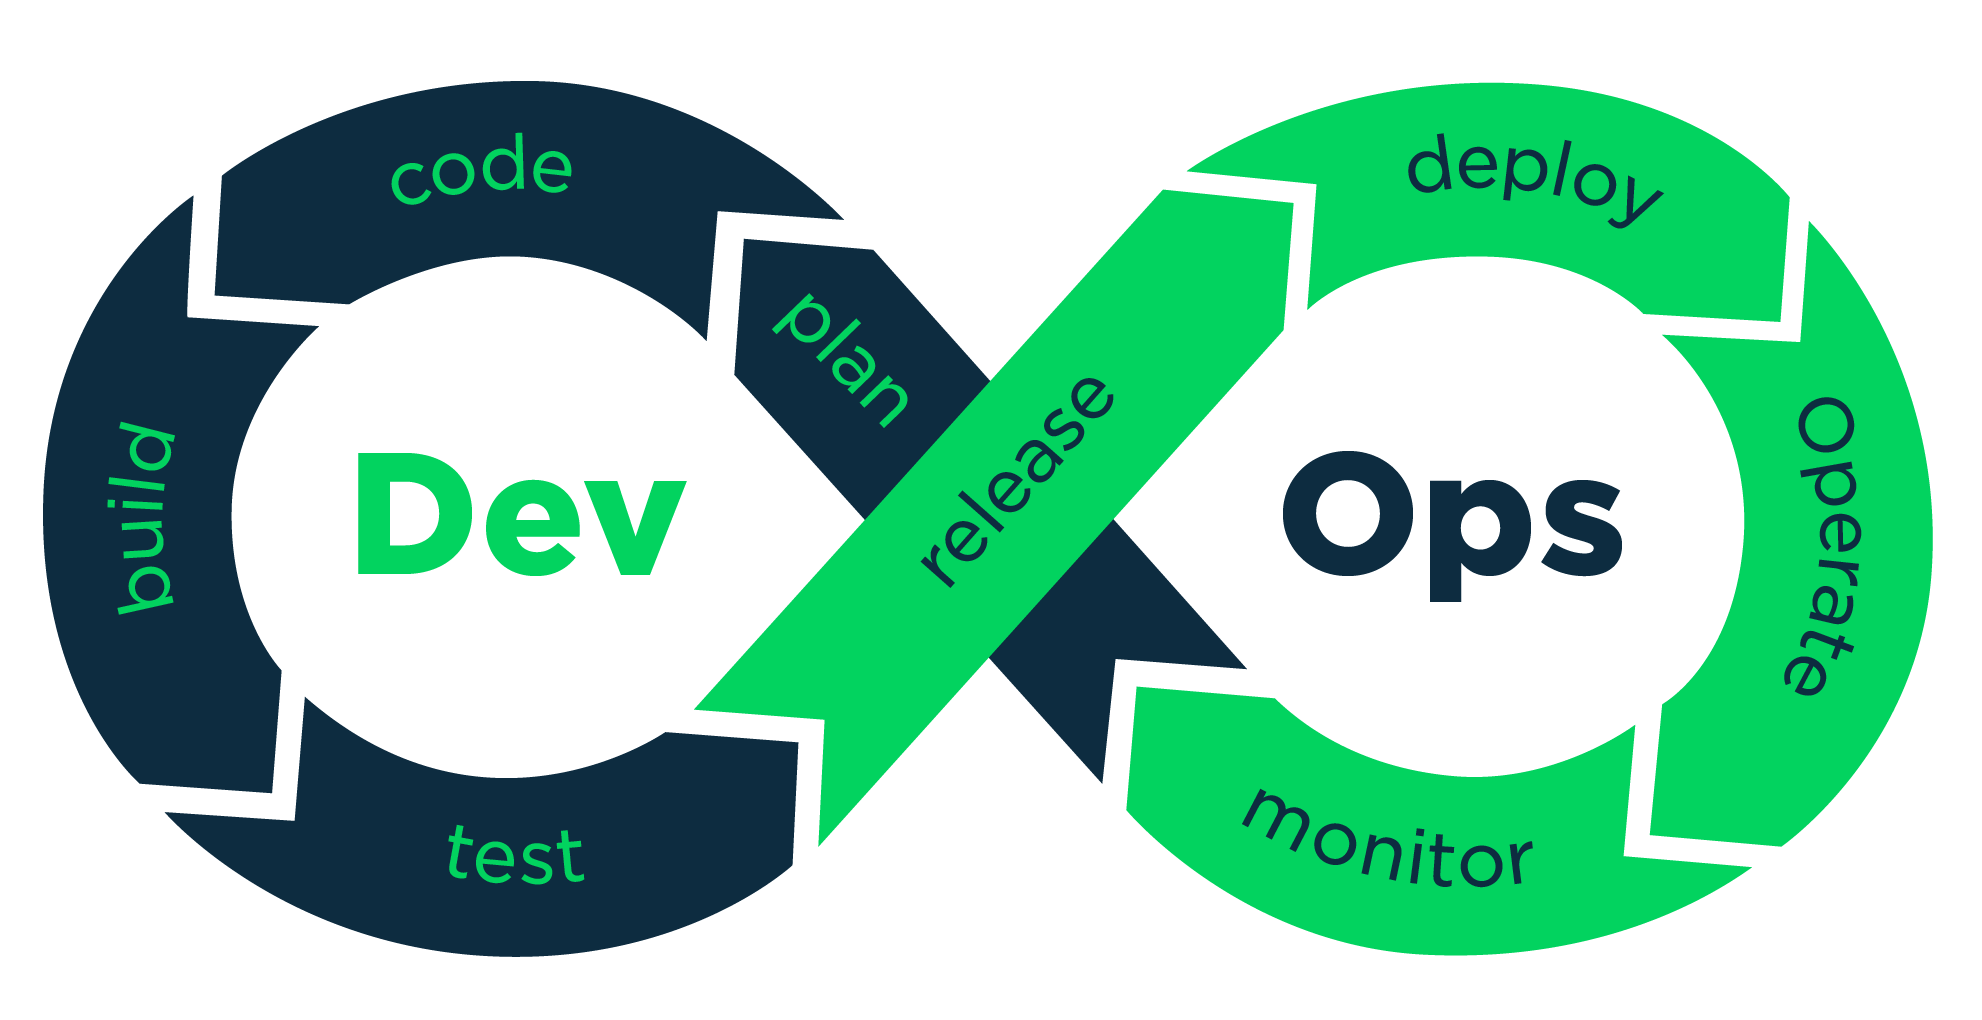
\includegraphics[width=100mm, keepaspectratio]{figures/devops.png}
    \caption{DevOps szemlélet a projektben}
    \label{fig:devops}
\end{figure}
%-----------------------------------------------------------------------------
